\documentclass[]{article}
\usepackage{lmodern}
\usepackage{amssymb,amsmath}
\usepackage{ifxetex,ifluatex}
\usepackage{fixltx2e} % provides \textsubscript
\ifnum 0\ifxetex 1\fi\ifluatex 1\fi=0 % if pdftex
  \usepackage[T1]{fontenc}
  \usepackage[utf8]{inputenc}
\else % if luatex or xelatex
  \ifxetex
    \usepackage{mathspec}
  \else
    \usepackage{fontspec}
  \fi
  \defaultfontfeatures{Ligatures=TeX,Scale=MatchLowercase}
\fi
% use upquote if available, for straight quotes in verbatim environments
\IfFileExists{upquote.sty}{\usepackage{upquote}}{}
% use microtype if available
\IfFileExists{microtype.sty}{%
\usepackage{microtype}
\UseMicrotypeSet[protrusion]{basicmath} % disable protrusion for tt fonts
}{}
\usepackage[margin=1in]{geometry}
\usepackage[unicode=true]{hyperref}
\hypersetup{
            pdftitle={Rock Lichen data from Sunset Crater},
            pdfauthor={M.K. Lau},
            pdfborder={0 0 0},
            breaklinks=true}
\urlstyle{same}  % don't use monospace font for urls
\usepackage{color}
\usepackage{fancyvrb}
\newcommand{\VerbBar}{|}
\newcommand{\VERB}{\Verb[commandchars=\\\{\}]}
\DefineVerbatimEnvironment{Highlighting}{Verbatim}{commandchars=\\\{\}}
% Add ',fontsize=\small' for more characters per line
\usepackage{framed}
\definecolor{shadecolor}{RGB}{248,248,248}
\newenvironment{Shaded}{\begin{snugshade}}{\end{snugshade}}
\newcommand{\KeywordTok}[1]{\textcolor[rgb]{0.13,0.29,0.53}{\textbf{{#1}}}}
\newcommand{\DataTypeTok}[1]{\textcolor[rgb]{0.13,0.29,0.53}{{#1}}}
\newcommand{\DecValTok}[1]{\textcolor[rgb]{0.00,0.00,0.81}{{#1}}}
\newcommand{\BaseNTok}[1]{\textcolor[rgb]{0.00,0.00,0.81}{{#1}}}
\newcommand{\FloatTok}[1]{\textcolor[rgb]{0.00,0.00,0.81}{{#1}}}
\newcommand{\ConstantTok}[1]{\textcolor[rgb]{0.00,0.00,0.00}{{#1}}}
\newcommand{\CharTok}[1]{\textcolor[rgb]{0.31,0.60,0.02}{{#1}}}
\newcommand{\SpecialCharTok}[1]{\textcolor[rgb]{0.00,0.00,0.00}{{#1}}}
\newcommand{\StringTok}[1]{\textcolor[rgb]{0.31,0.60,0.02}{{#1}}}
\newcommand{\VerbatimStringTok}[1]{\textcolor[rgb]{0.31,0.60,0.02}{{#1}}}
\newcommand{\SpecialStringTok}[1]{\textcolor[rgb]{0.31,0.60,0.02}{{#1}}}
\newcommand{\ImportTok}[1]{{#1}}
\newcommand{\CommentTok}[1]{\textcolor[rgb]{0.56,0.35,0.01}{\textit{{#1}}}}
\newcommand{\DocumentationTok}[1]{\textcolor[rgb]{0.56,0.35,0.01}{\textbf{\textit{{#1}}}}}
\newcommand{\AnnotationTok}[1]{\textcolor[rgb]{0.56,0.35,0.01}{\textbf{\textit{{#1}}}}}
\newcommand{\CommentVarTok}[1]{\textcolor[rgb]{0.56,0.35,0.01}{\textbf{\textit{{#1}}}}}
\newcommand{\OtherTok}[1]{\textcolor[rgb]{0.56,0.35,0.01}{{#1}}}
\newcommand{\FunctionTok}[1]{\textcolor[rgb]{0.00,0.00,0.00}{{#1}}}
\newcommand{\VariableTok}[1]{\textcolor[rgb]{0.00,0.00,0.00}{{#1}}}
\newcommand{\ControlFlowTok}[1]{\textcolor[rgb]{0.13,0.29,0.53}{\textbf{{#1}}}}
\newcommand{\OperatorTok}[1]{\textcolor[rgb]{0.81,0.36,0.00}{\textbf{{#1}}}}
\newcommand{\BuiltInTok}[1]{{#1}}
\newcommand{\ExtensionTok}[1]{{#1}}
\newcommand{\PreprocessorTok}[1]{\textcolor[rgb]{0.56,0.35,0.01}{\textit{{#1}}}}
\newcommand{\AttributeTok}[1]{\textcolor[rgb]{0.77,0.63,0.00}{{#1}}}
\newcommand{\RegionMarkerTok}[1]{{#1}}
\newcommand{\InformationTok}[1]{\textcolor[rgb]{0.56,0.35,0.01}{\textbf{\textit{{#1}}}}}
\newcommand{\WarningTok}[1]{\textcolor[rgb]{0.56,0.35,0.01}{\textbf{\textit{{#1}}}}}
\newcommand{\AlertTok}[1]{\textcolor[rgb]{0.94,0.16,0.16}{{#1}}}
\newcommand{\ErrorTok}[1]{\textcolor[rgb]{0.64,0.00,0.00}{\textbf{{#1}}}}
\newcommand{\NormalTok}[1]{{#1}}
\usepackage{graphicx,grffile}
\makeatletter
\def\maxwidth{\ifdim\Gin@nat@width>\linewidth\linewidth\else\Gin@nat@width\fi}
\def\maxheight{\ifdim\Gin@nat@height>\textheight\textheight\else\Gin@nat@height\fi}
\makeatother
% Scale images if necessary, so that they will not overflow the page
% margins by default, and it is still possible to overwrite the defaults
% using explicit options in \includegraphics[width, height, ...]{}
\setkeys{Gin}{width=\maxwidth,height=\maxheight,keepaspectratio}
\IfFileExists{parskip.sty}{%
\usepackage{parskip}
}{% else
\setlength{\parindent}{0pt}
\setlength{\parskip}{6pt plus 2pt minus 1pt}
}
\setlength{\emergencystretch}{3em}  % prevent overfull lines
\providecommand{\tightlist}{%
  \setlength{\itemsep}{0pt}\setlength{\parskip}{0pt}}
\setcounter{secnumdepth}{0}
% Redefines (sub)paragraphs to behave more like sections
\ifx\paragraph\undefined\else
\let\oldparagraph\paragraph
\renewcommand{\paragraph}[1]{\oldparagraph{#1}\mbox{}}
\fi
\ifx\subparagraph\undefined\else
\let\oldsubparagraph\subparagraph
\renewcommand{\subparagraph}[1]{\oldsubparagraph{#1}\mbox{}}
\fi

\title{Rock Lichen data from Sunset Crater}
\author{M.K. Lau}
\date{}

\begin{document}
\maketitle

\section{Analysis Summary}\label{analysis-summary}

\begin{itemize}
\tightlist
\item
  Dead trees and non-lichen species were removed from lichen community
  analyses.
\item
  Lichen communities were adequately sampled, based on species
  accumulation curves, with moth resistant trees accumulating slightly
  more lichen species.
\item
  Lichen communities (abundance, richness, diversity, composition) were
  significantly, generally negatively, affected by moth susceptibility.
\item
  Several tree variables, including light availability, leaf litter
  abundance and rock abundance, were impacted by moth susceptibility.
\item
  Analysis of causal pathways supported an indirect link between moth
  susceptibility and impacts on lichen communities via decreasing rock
  (i.e.~habitat) availability through increased leaf abscission and
  accumulation on rocks under trees.
\item
  These results support a genetically based link between intraspecific
  variation in susceptibility to an insect herbivore and community
  dynamics in an arid ecosystem.
\item
  Given the possible impacts of cliimate change on this system, this
  study supports the conclusion that community and ecosystem impacts
  need to be considered in an evolutionary context.
\end{itemize}

\begin{Shaded}
\begin{Highlighting}[]
\CommentTok{# 0. Supporting functions and libraries}
\NormalTok{## Support functions}

\NormalTok{dif <-}\StringTok{ }\NormalTok{function(x)\{}
    \NormalTok{out=x[}\DecValTok{1}\NormalTok{]}
    \NormalTok{for (i in }\DecValTok{2}\NormalTok{:}\KeywordTok{length}\NormalTok{(x))\{}
        \NormalTok{out=out-x[i]}
    \NormalTok{\}}
    \KeywordTok{return}\NormalTok{(out)}
\NormalTok{\}}

\NormalTok{## Libraries}
\NormalTok{my.libs <-}\StringTok{ }\KeywordTok{c}\NormalTok{(}\StringTok{"vegan"}\NormalTok{, }\StringTok{"ecodist"}\NormalTok{, }\StringTok{"knitr"}\NormalTok{, }\StringTok{"kableExtra"}\NormalTok{)}
\NormalTok{if (}\KeywordTok{any}\NormalTok{(!(my.libs %in%}\StringTok{ }\KeywordTok{installed.packages}\NormalTok{()[, }\DecValTok{1}\NormalTok{])))\{}
    \KeywordTok{sapply}\NormalTok{(my.libs[!(my.libs %in%}\StringTok{ }\KeywordTok{installed.packages}\NormalTok{()[, }\DecValTok{1}\NormalTok{])], }
           \NormalTok{install.packages)}
\NormalTok{\}else\{\}}
\KeywordTok{sapply}\NormalTok{(my.libs, require, }\DataTypeTok{character.only =} \OtherTok{TRUE}\NormalTok{)}
\end{Highlighting}
\end{Shaded}

\section{Load Data}\label{load-data}

The following are variable descriptions (Variable, Type, Range,
Definition):

\begin{itemize}
\tightlist
\item
  Moth,categorical,0 or 1,Was the tree susceptible (0) or resistant (1)
  to moth attack?
\item
  Live/Dead,categorical,0 or 1,Was the tree dead (0) or alive (1)?
\item
  Litter \%,continuous,0 to 100,Percent cover inside quadrat
\item
  Rocks \textgreater{} 3cm? \%,continuous,0 to 100,Percent cover of
  rocks \textgreater{} 3cm? inside quadrat
\item
  Rocks \textless{} 3cm? \%,continuous,0 to 100,Percent cover of rocks
  \textless{} 3cm? inside quadrat
\item
  Shrubs \%,continuous,0 to 100,Percent cover of shrubs inside quadrat
\item
  Grass \%,continuous,0 to 100,Percent cover of grass inside quadrat
\item
  Branches \%,continuous,0 to 100,Percent cover of branches on ground
  inside quadrat
\item
  Distance,continuous,0 to 100,``Distance from main trunk, converted to
  percent of crown radius at that azimuth''
\item
  Azimuth,continuous,0 to 360,Compass direction from main trunk
\item
  Slope,continuous,0 to 90,Topographical steepness
\item
  Aspect,continuous,0 to 360,Compass direction of slope
\item
  Light,continuous,,Amount of light available to epiliths
\end{itemize}

\begin{Shaded}
\begin{Highlighting}[]
\NormalTok{## Data are in ../data/scrl}
\NormalTok{l.dat <-}\StringTok{ }\KeywordTok{read.csv}\NormalTok{(}\StringTok{"../data/scrl/spp_env_combined.csv"}\NormalTok{)}

\NormalTok{## Summary of data}
\KeywordTok{summary}\NormalTok{(l.dat)}

\NormalTok{## remove dead trees}
\NormalTok{l.dat <-}\StringTok{ }\NormalTok{l.dat[l.dat[, }\StringTok{"Live.Dead"}\NormalTok{] !=}\StringTok{ }\DecValTok{0}\NormalTok{, ]}

\NormalTok{## Lichen species list}
\NormalTok{spp.l <-}\StringTok{ }\KeywordTok{c}\NormalTok{(}\StringTok{"Acacon"}\NormalTok{, }\StringTok{"Acasup"}\NormalTok{, }\StringTok{"Acaobp"}\NormalTok{, }\StringTok{"Sterile.sp"}\NormalTok{, }\StringTok{"Brown.cr"}\NormalTok{,}
\StringTok{"Lobalp"}\NormalTok{, }\StringTok{"Canros"}\NormalTok{, }\StringTok{"Calare"}\NormalTok{, }\StringTok{"Phydub"}\NormalTok{, }\StringTok{"Rhichr"}\NormalTok{, }\StringTok{"Xanlin"}\NormalTok{, }\StringTok{"Xanpli"}\NormalTok{,}
\StringTok{"Xanele"}\NormalTok{, }\StringTok{"GrBr.cr"}\NormalTok{, }\StringTok{"Gray.cr"}\NormalTok{)}
\NormalTok{spp.moss <-}\StringTok{ }\KeywordTok{c}\NormalTok{(}\StringTok{"Synrur"}\NormalTok{, }\StringTok{"Cerpur.Bryarg"}\NormalTok{)}

\NormalTok{## Create a community matrix}
\NormalTok{com <-}\StringTok{ }\NormalTok{l.dat[, }\KeywordTok{colnames}\NormalTok{(l.dat) %in%}\StringTok{ }\NormalTok{spp.l]}
\NormalTok{com.moss <-}\StringTok{ }\NormalTok{l.dat[, }\KeywordTok{colnames}\NormalTok{(l.dat) %in%}\StringTok{ }\NormalTok{spp.moss]}

\NormalTok{## Add the tree labels to the rownames}
\KeywordTok{rownames}\NormalTok{(com) <-}\StringTok{ }\KeywordTok{paste}\NormalTok{(l.dat[, }\StringTok{"Moth"}\NormalTok{], l.dat[, }\StringTok{"Tree.pairs"}\NormalTok{], }\DataTypeTok{sep =} \StringTok{"_"}\NormalTok{)}
\KeywordTok{rownames}\NormalTok{(com.moss) <-}\StringTok{ }\KeywordTok{paste}\NormalTok{(l.dat[, }\StringTok{"Moth"}\NormalTok{], l.dat[, }\StringTok{"Tree.pairs"}\NormalTok{], }\DataTypeTok{sep =} \StringTok{"_"}\NormalTok{)}
\KeywordTok{rownames}\NormalTok{(l.dat) <-}\StringTok{ }\KeywordTok{paste}\NormalTok{(l.dat[, }\StringTok{"Moth"}\NormalTok{], l.dat[, }\StringTok{"Tree.pairs"}\NormalTok{], }\DataTypeTok{sep =} \StringTok{"_"}\NormalTok{)}
\end{Highlighting}
\end{Shaded}

\section{Species accumulation}\label{species-accumulation}

Are the communities on each tree type adequately sampled?

\begin{Shaded}
\begin{Highlighting}[]
\NormalTok{spa.all <-}\StringTok{ }\KeywordTok{specaccum}\NormalTok{(com)}
\NormalTok{spa.res <-}\StringTok{ }\KeywordTok{specaccum}\NormalTok{(com[l.dat[, }\StringTok{"Moth"}\NormalTok{] ==}\StringTok{ }\DecValTok{0}\NormalTok{, ])}
\NormalTok{spa.sus <-}\StringTok{ }\KeywordTok{specaccum}\NormalTok{(com[l.dat[, }\StringTok{"Moth"}\NormalTok{] ==}\StringTok{ }\DecValTok{1}\NormalTok{, ])}

\KeywordTok{plot}\NormalTok{(spa.all,}
     \DataTypeTok{ylim =} \KeywordTok{c}\NormalTok{(}\DecValTok{0}\NormalTok{, }\DecValTok{20}\NormalTok{),}
     \DataTypeTok{xlab =} \StringTok{"Cumulative Trees Sampled"}\NormalTok{,}
     \DataTypeTok{ylab =} \StringTok{"Lichen Species Observed"}\NormalTok{, }
     \DataTypeTok{col =} \StringTok{"grey"}\NormalTok{, }\DataTypeTok{ci.col =} \StringTok{'lightgrey'}\NormalTok{, }\DataTypeTok{ci.type =} \StringTok{"poly"}\NormalTok{, }\DataTypeTok{ci.lty =} \DecValTok{0}\NormalTok{)}
\KeywordTok{plot}\NormalTok{(spa.res, }\DataTypeTok{ci.col =} \StringTok{"black"}\NormalTok{, }\DataTypeTok{ci.type =} \StringTok{"bar"}\NormalTok{, }\DataTypeTok{lty =} \DecValTok{1}\NormalTok{, }\DataTypeTok{add =} \OtherTok{TRUE}\NormalTok{, }\DataTypeTok{ci.lty =} \DecValTok{1}\NormalTok{)}
\KeywordTok{plot}\NormalTok{(spa.sus, }\DataTypeTok{ci.col =} \StringTok{"black"}\NormalTok{, }\DataTypeTok{ci.type =} \StringTok{"bar"}\NormalTok{, }\DataTypeTok{lty =} \DecValTok{3}\NormalTok{, }\DataTypeTok{add =} \OtherTok{TRUE}\NormalTok{, }\DataTypeTok{ci.lty =} \DecValTok{3}\NormalTok{)}
\KeywordTok{legend}\NormalTok{(}\StringTok{"bottomright"}\NormalTok{, }
       \DataTypeTok{legend =} \KeywordTok{c}\NormalTok{(}\StringTok{"All"}\NormalTok{, }\StringTok{"Resistant"}\NormalTok{, }\StringTok{"Susceptible"}\NormalTok{), }
       \DataTypeTok{lty =} \KeywordTok{c}\NormalTok{(}\DecValTok{1}\NormalTok{, }\DecValTok{1}\NormalTok{, }\DecValTok{3}\NormalTok{), }\DataTypeTok{lwd =} \KeywordTok{c}\NormalTok{(}\DecValTok{5}\NormalTok{, }\DecValTok{2}\NormalTok{, }\DecValTok{2}\NormalTok{), }\DataTypeTok{col =} \KeywordTok{c}\NormalTok{(}\StringTok{"lightgrey"}\NormalTok{, }\StringTok{"black"}\NormalTok{, }\StringTok{"black"}\NormalTok{))}
\end{Highlighting}
\end{Shaded}

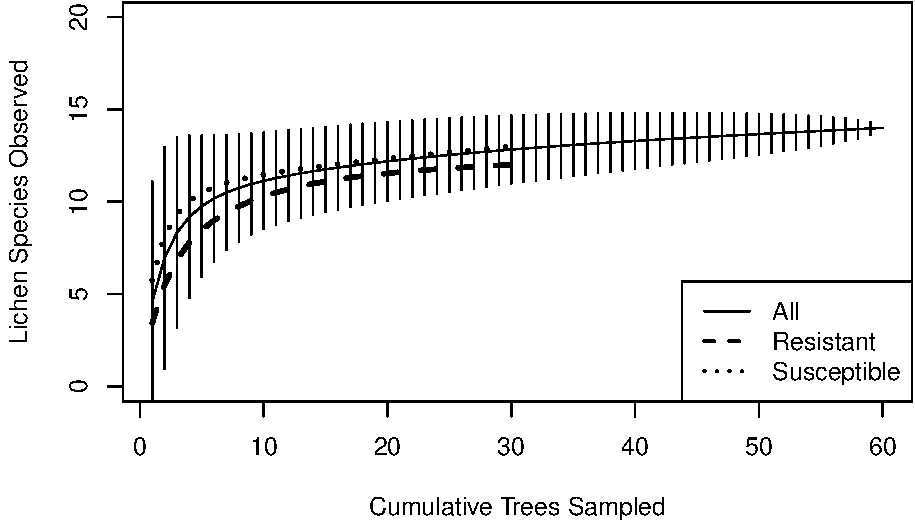
\includegraphics{rln_files/figure-latex/specacum-1.pdf}

\section{Moth trees have different
microenvironments}\label{moth-trees-have-different-microenvironments}

\begin{itemize}
\tightlist
\item
  paired t-tests
\end{itemize}

\section{Moth trees have different lichen communities (FIGURE ch.plot A,
R,
H)}\label{moth-trees-have-different-lichen-communities-figure-ch.plot-a-r-h}

less abundant and diverse (paired t-tests, in text)

\begin{Shaded}
\begin{Highlighting}[]
\NormalTok{abun <-}\StringTok{ }\KeywordTok{apply}\NormalTok{(com, }\DecValTok{1}\NormalTok{, sum)}
\NormalTok{rich <-}\StringTok{ }\KeywordTok{apply}\NormalTok{(com, }\DecValTok{1}\NormalTok{, function(x) }\KeywordTok{sum}\NormalTok{(}\KeywordTok{sign}\NormalTok{(x)))}
\NormalTok{shan <-}\StringTok{ }\KeywordTok{apply}\NormalTok{(com, }\DecValTok{1}\NormalTok{, diversity, }\DataTypeTok{index =} \StringTok{"shannon"}\NormalTok{)}
\NormalTok{tt.a <-}\StringTok{ }\KeywordTok{t.test}\NormalTok{(}\KeywordTok{tapply}\NormalTok{(abun, l.dat[, }\StringTok{"Tree.pairs"}\NormalTok{], diff))}
\NormalTok{tt.r <-}\StringTok{ }\KeywordTok{t.test}\NormalTok{(}\KeywordTok{tapply}\NormalTok{(rich, l.dat[, }\StringTok{"Tree.pairs"}\NormalTok{], diff))}
\NormalTok{tt.h <-}\StringTok{ }\KeywordTok{t.test}\NormalTok{(}\KeywordTok{tapply}\NormalTok{(shan, l.dat[, }\StringTok{"Tree.pairs"}\NormalTok{], diff))}
\NormalTok{tt.arh <-}\StringTok{ }\KeywordTok{do.call}\NormalTok{(rbind, }
                  \KeywordTok{list}\NormalTok{(}\DataTypeTok{a =} \KeywordTok{unlist}\NormalTok{(tt.a), }\DataTypeTok{r =} \KeywordTok{unlist}\NormalTok{(tt.r), }\DataTypeTok{h =} \KeywordTok{unlist}\NormalTok{(tt.h)))}
\KeywordTok{data.frame}\NormalTok{(tt.arh)}
\end{Highlighting}
\end{Shaded}

\begin{verbatim}
##         statistic.t parameter.df             p.value          conf.int1
## a -2.35680534636893           29  0.0253991007560338  -2.89259563276878
## r -2.83579994251995           29 0.00824742800912124  -3.95880113980294
## h -2.43278934693583           29  0.0213834528180339 -0.783514237345595
##             conf.int2 estimate.mean.of.x null.value.mean            stderr
## a  -0.204737700564557  -1.54866666666667               0 0.657104189386137
## r  -0.641198860197055               -2.3               0 0.811058624239964
## h -0.0678109108683952 -0.425662574106995               0 0.174968940341312
##   alternative            method                                 data.name
## a   two.sided One Sample t-test tapply(abun, l.dat[, "Tree.pairs"], diff)
## r   two.sided One Sample t-test tapply(rich, l.dat[, "Tree.pairs"], diff)
## h   two.sided One Sample t-test tapply(shan, l.dat[, "Tree.pairs"], diff)
\end{verbatim}

composition is different (PERMANOVA, in text and supplement)

\begin{Shaded}
\begin{Highlighting}[]
\NormalTok{com.ds <-}\StringTok{ }\KeywordTok{cbind}\NormalTok{(com, }\DataTypeTok{ds =} \KeywordTok{rep}\NormalTok{(}\FloatTok{0.0001}\NormalTok{, }\KeywordTok{nrow}\NormalTok{(com)))}
\NormalTok{com.ds.rel <-}\StringTok{ }\KeywordTok{apply}\NormalTok{(com, }\DecValTok{2}\NormalTok{, function(x) x/}\KeywordTok{max}\NormalTok{(x))}
\NormalTok{com.ds.rel <-}\StringTok{ }\KeywordTok{cbind}\NormalTok{(com.ds.rel, }\DataTypeTok{ds =} \KeywordTok{rep}\NormalTok{(}\FloatTok{0.0001}\NormalTok{, }\KeywordTok{nrow}\NormalTok{(com)))}
\NormalTok{com.ds.rel[}\KeywordTok{is.na}\NormalTok{(com.ds.rel)] <-}\StringTok{ }\DecValTok{0}

\KeywordTok{set.seed}\NormalTok{(}\DecValTok{123}\NormalTok{)}
\NormalTok{ptab.moth <-}\StringTok{ }\KeywordTok{adonis2}\NormalTok{(com.ds~}\StringTok{ }\NormalTok{Moth, }\DataTypeTok{data =} \NormalTok{l.dat, }
                    \DataTypeTok{strata =} \NormalTok{l.dat[, }\StringTok{"Tree.pairs"}\NormalTok{], }
                    \DataTypeTok{by =} \StringTok{"margin"}\NormalTok{, }\DataTypeTok{nperm =} \DecValTok{100000}\NormalTok{)}
\KeywordTok{set.seed}\NormalTok{(}\DecValTok{123}\NormalTok{)}
\NormalTok{ptab.moth.rel <-}\StringTok{ }\KeywordTok{adonis2}\NormalTok{(com.ds.rel ~}\StringTok{ }\NormalTok{Moth, }\DataTypeTok{data =} \NormalTok{l.dat, }
                         \DataTypeTok{strata =} \NormalTok{l.dat[, }\StringTok{"Tree.pairs"}\NormalTok{], }
                         \DataTypeTok{by =} \StringTok{"margin"}\NormalTok{, }\DataTypeTok{nperm =} \DecValTok{100000}\NormalTok{)}

\KeywordTok{kable}\NormalTok{(ptab.moth)}
\end{Highlighting}
\end{Shaded}

\begin{tabular}{l|r|r|r|r|r}
\hline
  & Df & SumOfSqs & R2 & F & Pr(>F)\\
\hline
Moth & 1 & 0.8281197 & 0.0389381 & 2.349914 & 0.023\\
\hline
Residual & 58 & 20.4394472 & 0.9610619 & NA & NA\\
\hline
Total & 59 & 21.2675669 & 1.0000000 & NA & NA\\
\hline
\end{tabular}

\begin{Shaded}
\begin{Highlighting}[]
\KeywordTok{kable}\NormalTok{(ptab.moth.rel)}
\end{Highlighting}
\end{Shaded}

\begin{tabular}{l|r|r|r|r|r}
\hline
  & Df & SumOfSqs & R2 & F & Pr(>F)\\
\hline
Moth & 1 & 0.8836864 & 0.0409591 & 2.477087 & 0.02\\
\hline
Residual & 58 & 20.6911630 & 0.9590409 & NA & NA\\
\hline
Total & 59 & 21.5748495 & 1.0000000 & NA & NA\\
\hline
\end{tabular}

three main species were reduced by moths (FDR paired t-tests, in text +
supplement)

\begin{Shaded}
\begin{Highlighting}[]
\NormalTok{ind.spp <-}\StringTok{ }\KeywordTok{lapply}\NormalTok{(com, function(x, p) }\KeywordTok{t.test}\NormalTok{(}\KeywordTok{tapply}\NormalTok{(x, p, diff)), }\DataTypeTok{p =} \NormalTok{l.dat[, }\StringTok{"Tree.pairs"}\NormalTok{])}
\NormalTok{isp <-}\StringTok{ }\KeywordTok{apply}\NormalTok{(}\KeywordTok{do.call}\NormalTok{(rbind, }\KeywordTok{lapply}\NormalTok{(ind.spp, unlist)), }\DecValTok{2}\NormalTok{, as.numeric)}
\end{Highlighting}
\end{Shaded}

\begin{verbatim}
## Warning in apply(do.call(rbind, lapply(ind.spp, unlist)), 2, as.numeric): NAs
## introduced by coercion

## Warning in apply(do.call(rbind, lapply(ind.spp, unlist)), 2, as.numeric): NAs
## introduced by coercion

## Warning in apply(do.call(rbind, lapply(ind.spp, unlist)), 2, as.numeric): NAs
## introduced by coercion
\end{verbatim}

\begin{Shaded}
\begin{Highlighting}[]
\KeywordTok{rownames}\NormalTok{(isp) <-}\StringTok{ }\KeywordTok{names}\NormalTok{(ind.spp)}
\NormalTok{isp[, }\StringTok{"p.value"}\NormalTok{] <-}\StringTok{ }\KeywordTok{p.adjust}\NormalTok{(isp[, }\StringTok{"p.value"}\NormalTok{], }\DataTypeTok{method =} \StringTok{"fdr"}\NormalTok{)}
\NormalTok{isp <-}\StringTok{ }\NormalTok{isp[}\KeywordTok{order}\NormalTok{(isp[, }\StringTok{"p.value"}\NormalTok{]), ]}
\KeywordTok{head}\NormalTok{(isp[, }\DecValTok{1}\NormalTok{:}\DecValTok{3}\NormalTok{])}
\end{Highlighting}
\end{Shaded}

\begin{verbatim}
##        statistic.t parameter.df    p.value
## Acacon   -3.377629           29 0.01390405
## Acasup   -3.242091           29 0.01390405
## Canros   -3.581884           29 0.01390405
## Lobalp   -2.041361           29 0.17642430
## Phydub   -1.922619           29 0.18031798
## Calare   -1.607607           29 0.22424946
\end{verbatim}

\section{Litter covering rocks was the main driver (FIGURE =
ORDINATION)}\label{litter-covering-rocks-was-the-main-driver-figure-ordination}

light not litter predicted lichen composition (PERMANOVA, table 3,
Ordination)

\begin{Shaded}
\begin{Highlighting}[]
\KeywordTok{set.seed}\NormalTok{(}\DecValTok{123}\NormalTok{)}
\NormalTok{ptab.env <-}\StringTok{ }\KeywordTok{adonis2}\NormalTok{(com.ds ~}\StringTok{  }\NormalTok{Light...average +}\StringTok{ }\NormalTok{Litter.., }\DataTypeTok{data =} \NormalTok{l.dat, }
                   \DataTypeTok{strata =} \NormalTok{l.dat[, }\StringTok{"Tree.pairs"}\NormalTok{],  }
                   \DataTypeTok{by =} \StringTok{"margin"}\NormalTok{, }\DataTypeTok{nperm =} \DecValTok{100000}\NormalTok{)}
\KeywordTok{kable}\NormalTok{(ptab.env)}
\end{Highlighting}
\end{Shaded}

\begin{tabular}{l|r|r|r|r|r}
\hline
  & Df & SumOfSqs & R2 & F & Pr(>F)\\
\hline
Light...average & 1 & 0.4114804 & 0.0193478 & 1.225652 & 0.240\\
\hline
Litter.. & 1 & 1.0095951 & 0.0474711 & 3.007221 & 0.007\\
\hline
Residual & 57 & 19.1362475 & 0.8997855 & NA & NA\\
\hline
Total & 59 & 21.2675669 & 1.0000000 & NA & NA\\
\hline
\end{tabular}

\begin{Shaded}
\begin{Highlighting}[]
\NormalTok{nmds.out <-}\StringTok{ }\KeywordTok{nmds}\NormalTok{(}\KeywordTok{vegdist}\NormalTok{(com.ds), }\DecValTok{2}\NormalTok{, }\DecValTok{2}\NormalTok{)}
\NormalTok{ord <-}\StringTok{ }\KeywordTok{nmds.min}\NormalTok{(nmds.out, }\DataTypeTok{dims =} \DecValTok{2}\NormalTok{)}
\end{Highlighting}
\end{Shaded}

\begin{verbatim}
## Minimum stress for given dimensionality:  0.2164016 
## r^2 for minimum stress configuration:  0.6474944
\end{verbatim}

\begin{Shaded}
\begin{Highlighting}[]
\NormalTok{ord.pch <-}\StringTok{ }\KeywordTok{c}\NormalTok{(}\StringTok{"R"}\NormalTok{, }\StringTok{"S"}\NormalTok{)[(l.dat[, }\StringTok{"Moth"}\NormalTok{] +}\StringTok{ }\DecValTok{1}\NormalTok{)]}
\KeywordTok{plot}\NormalTok{(X2~}\StringTok{ }\NormalTok{X1, }\DataTypeTok{data =} \NormalTok{ord, }\DataTypeTok{pch =} \NormalTok{ord.pch)}
\end{Highlighting}
\end{Shaded}

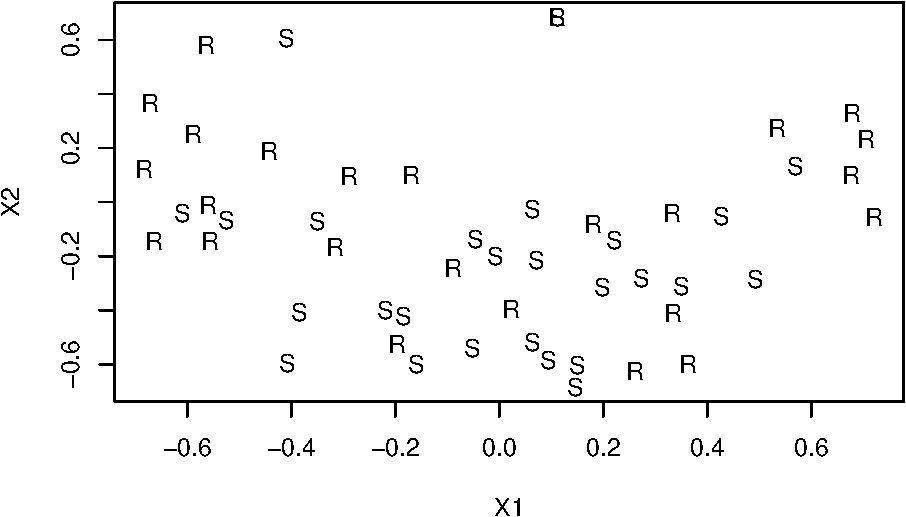
\includegraphics{rln_files/figure-latex/ord-com-plot-1.pdf}

litter not light was correlated with large rocks (dist cor, in text)

\begin{Shaded}
\begin{Highlighting}[]
\KeywordTok{cor.test}\NormalTok{(}\KeywordTok{tapply}\NormalTok{(l.dat[, }\StringTok{"Big.rocks.."}\NormalTok{], l.dat[, }\StringTok{"Tree.pairs"}\NormalTok{], diff),}
         \KeywordTok{tapply}\NormalTok{(l.dat[, }\StringTok{"Litter.."}\NormalTok{], l.dat[, }\StringTok{"Tree.pairs"}\NormalTok{], diff))}
\end{Highlighting}
\end{Shaded}

\begin{verbatim}
## 
##  Pearson's product-moment correlation
## 
## data:  tapply(l.dat[, "Big.rocks.."], l.dat[, "Tree.pairs"], diff) and tapply(l.dat[, "Litter.."], l.dat[, "Tree.pairs"], diff)
## t = -11.106, df = 28, p-value = 9.054e-12
## alternative hypothesis: true correlation is not equal to 0
## 95 percent confidence interval:
##  -0.9530598 -0.8039735
## sample estimates:
##        cor 
## -0.9027609
\end{verbatim}

\begin{Shaded}
\begin{Highlighting}[]
\KeywordTok{cor.test}\NormalTok{(}\KeywordTok{tapply}\NormalTok{(l.dat[, }\StringTok{"Big.rocks.."}\NormalTok{], l.dat[, }\StringTok{"Tree.pairs"}\NormalTok{], diff),}
         \KeywordTok{tapply}\NormalTok{(l.dat[, }\StringTok{"Light...average"}\NormalTok{], l.dat[, }\StringTok{"Tree.pairs"}\NormalTok{], diff))}
\end{Highlighting}
\end{Shaded}

\begin{verbatim}
## 
##  Pearson's product-moment correlation
## 
## data:  tapply(l.dat[, "Big.rocks.."], l.dat[, "Tree.pairs"], diff) and tapply(l.dat[, "Light...average"], l.dat[, "Tree.pairs"], diff)
## t = 0.71624, df = 28, p-value = 0.4798
## alternative hypothesis: true correlation is not equal to 0
## 95 percent confidence interval:
##  -0.2376184  0.4716125
## sample estimates:
##       cor 
## 0.1341335
\end{verbatim}

\begin{Shaded}
\begin{Highlighting}[]
\KeywordTok{cor.test}\NormalTok{(}\KeywordTok{tapply}\NormalTok{(l.dat[, }\StringTok{"Litter.."}\NormalTok{], l.dat[, }\StringTok{"Tree.pairs"}\NormalTok{], diff),}
         \KeywordTok{tapply}\NormalTok{(l.dat[, }\StringTok{"Light...average"}\NormalTok{], l.dat[, }\StringTok{"Tree.pairs"}\NormalTok{], diff))}
\end{Highlighting}
\end{Shaded}

\begin{verbatim}
## 
##  Pearson's product-moment correlation
## 
## data:  tapply(l.dat[, "Litter.."], l.dat[, "Tree.pairs"], diff) and tapply(l.dat[, "Light...average"], l.dat[, "Tree.pairs"], diff)
## t = -0.92053, df = 28, p-value = 0.3652
## alternative hypothesis: true correlation is not equal to 0
## 95 percent confidence interval:
##  -0.5007401  0.2013096
## sample estimates:
##        cor 
## -0.1713898
\end{verbatim}

\begin{Shaded}
\begin{Highlighting}[]
\KeywordTok{cor.test}\NormalTok{(}\KeywordTok{tapply}\NormalTok{(l.dat[, }\StringTok{"Litter.."}\NormalTok{], l.dat[, }\StringTok{"Tree.pairs"}\NormalTok{], diff),}
         \KeywordTok{tapply}\NormalTok{(l.dat[, }\StringTok{"Light...average"}\NormalTok{], l.dat[, }\StringTok{"Tree.pairs"}\NormalTok{], diff))}
\end{Highlighting}
\end{Shaded}

\begin{verbatim}
## 
##  Pearson's product-moment correlation
## 
## data:  tapply(l.dat[, "Litter.."], l.dat[, "Tree.pairs"], diff) and tapply(l.dat[, "Light...average"], l.dat[, "Tree.pairs"], diff)
## t = -0.92053, df = 28, p-value = 0.3652
## alternative hypothesis: true correlation is not equal to 0
## 95 percent confidence interval:
##  -0.5007401  0.2013096
## sample estimates:
##        cor 
## -0.1713898
\end{verbatim}

\end{document}
